\subsection{Pile-up correction}
\label{subsection: charged particle density, pile-up}
%At the LHCb detector pile-up is defined as the average number of proton-proton interactions ($n$) in visible events. 

The Pile-Up is the number of proton interactions corresponding to a bunch crossing instance. A bunch crossing consisting of multiple proton interactions will associate all interactions to the same event. In order to calculate the charged particle density associated to a single proton-proton interaction a correction is applied to remove the effects of pile-up. The amount of pile expected in a data sample is related to the number visible proton-proton interactions ($n$) per bunch crossing, this follows a Poisson distribution given by equation \ref{equation: number of visible proton-proton interactions per bunch crossing}. 

\begin{equation}
	P(n; \mu) = \frac{\mu^n e^{-\mu}}{n!}
	\label{equation: number of visible proton-proton interactions per bunch crossing}
\end{equation}

where $\mu$ is the expected number of visible proton-proton interactions per bunch crossing. The value of $\mu$ for a dataset can be calculated by plotting the distribution of the time passed between consecutive events ($g(\Delta t)$) and fitting it to equation \ref{equation: delta t},

\begin{equation}
	g(\Delta t) = e^{-\mu\cdot k \cdot f \cdot \Delta t}
	\label{equation: delta t}
\end{equation}

where $k$ is the number of colliding bunches (1 for magnet down data and 2 for magnet up data) and $f$ is the LHC revolution frequency (11.246 kHz for data collected in 2010). Fitting the distribution (see figure \ref{fig: delta t distribution}) gives a $\mu$ is of 0.0261 for magnet down data and 0.0066 for magnet up data in 2010. % corresponding to a probability of seeing another interaction ($\sim \mu/2$) of approximately 1\%. %Due to the smallness of the probability of pile-up events, its effect on the charged particle density is negligible.

\begin{figure}[h]
	\centering
	\begin{subfigure}{0.49\textwidth}
		\centering
		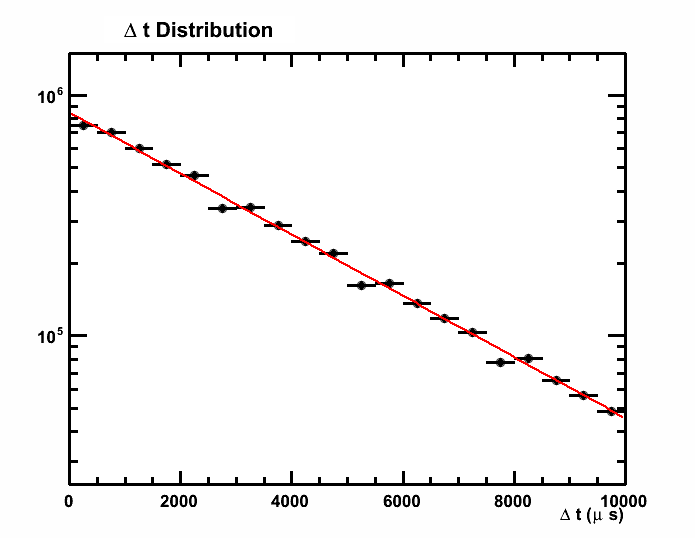
\includegraphics[width=\textwidth]{/Users/admin/Dropbox/PhD/Thesis/Chapters/multiplicity/images/delta_t_distribution_down_no_event_selection.png}
		\caption{Magnet Down}
	\end{subfigure}
	\begin{subfigure}{0.49\textwidth}
		\centering
		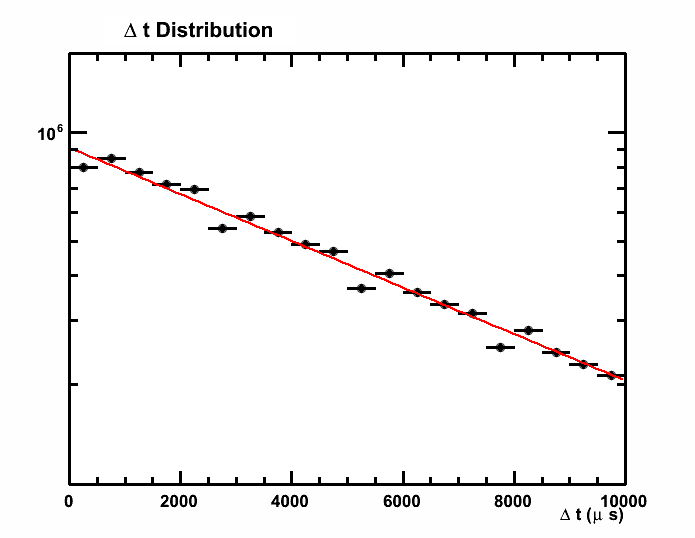
\includegraphics[width=\textwidth]{/Users/admin/Dropbox/PhD/Thesis/Chapters/multiplicity/images/delta_t_distribution_up_no_event_selection.png}
		\caption{Magnet Up}
	\end{subfigure}
	\caption{Distribution of the time between events with at least one track reconstructed}
	\label{fig: delta t distribution}
\end{figure}

Introducing a trigger condition that accepts only events with visible interactions gives a probability distribution of observing $n$ interactions ($1 \le n \le \infty$) with an expected number of interactions $\mu_1$ described by a renormalised zero suppressed Poisson distribution.

\begin{equation}
	P_1(n; \mu_1) = \frac{P(n; \mu)}{1 - P(0; \mu)} \,\,\,\,\,\,\,\,\,\,\,\,\,\,\,\,\,\,\,\,\,\,\,\, \mathrm{for} \,\, 1 \le n \le \infty
\end{equation}

The expectation value $\mu_1$ that describes the expected number of visible interactions in triggered events, i.e. pile-up is given by,

\begin{equation}
	\mu_1 = \frac{\sum^{\infty}_{n=1}{n\cdot P(n; \mu)}}{1 - P(0; \mu)} = \frac{\sum^{\infty}_{k=0}{n\cdot P(n; \mu)}}{1-e^{-\mu}} = \frac{\mu}{1 - e^{-\mu}}
\end{equation}

For small values of $\mu$ the pile-up can be expressed as the following expansion,

\begin{equation}
	\mu_1 \approx \frac{\mu}{1 - (1 - \mu + \mu^2/2)} \approx 1 + \frac{\mu}{2}
	\label{equation: mu approximation}
\end{equation}

To correct the particle density distributions the number of events are renormalised to include events including two proton-proton interactions, this is given by,

\begin{equation}
	N^\mathrm{total}_{ev} = \mu_1 \cdot N_\mathrm{ev} = N_\mathrm{ev}(1 + \frac{\mu}{2})
\end{equation}

This corresponds to a decrease in the charged particle density of 1.3\% for magnet down data and 0.33\% for magnet up data.

%\begin{equation}
%	N_\mathrm{int}^\mathrm{total} = \frac{p_1}{p_\mathrm{total}} \cdot N_\mathrm{ev} + 2 \frac{p_2}{p_\mathrm{total}} \cdot N_\mathrm{ev}
%\end{equation}
%
%where $p_n$ is described by,
%
%\begin{equation*}
%	p_n = \frac{\mu^n e^{-\mu}}{n!}
%\end{equation*}

%To calculate the multiplicity distribution for events with single proton-proton interactions it is required to correct for effects due to the pile-up. The observed multiplicity distribution ($\theta$) is modelled as the convolution of single proton-proton interaction distributions ($\phi$), given by,
%
%\begin{equation}
%	\theta(n) = \frac{1}{\sum_{k=1}^{\infty} P(k)} \sum_{k=1}^{\infty}P(k)\phi_k(n)
%\end{equation}
%
%with,
%\begin{equation*}
%	\phi_k = \phi \ast \phi ... \ast \phi \mathrm{\,\,\,\,\,} k \mathrm{\,times}
%\end{equation*}
%
%For small values of $\mu$ it is sufficient to consider only the first two terms. The expression for the pile-up ($\mu_1$) in this regime can be expanded as,
%\begin{equation}
%	\mu_1 \approx \frac{\mu}{1 - (1 - \mu + \mu^2/2)}
%\end{equation}
%or,
%\begin{equation}
%	\mu_1 \approx 1 + \frac{\mu}{2}
%\end{equation}
%
%The expression for the observed distribution in terms of convolutions of single proton-proton interaction distributions approximates to,
%
%\begin{equation}
%	\theta(n) \approx \frac{P(1)\phi(n) + P(2)\phi_2(n)}{P(1) + P(2)} = \frac{\phi(n) + (\mu/2)\phi_2(n)}{1 + \mu/2}
%\end{equation}
%
%In terms of the single proton-proton interaction distribution $\phi$ this is,
%
%\begin{equation}
%	\phi(n) = (1 + \frac{\mu}{2})\theta(n) - \frac{\mu}{2}\phi_2(n)
%\end{equation}
%
%The form of this equation suggests an iterative approach to calculating the solution with,
%
%\begin{equation}
%	\phi^{i+1}(n) = (1 + \frac{\mu}{2})\theta(n) - \frac{\mu}{2}\phi_2^{i}(n) \mathrm{\,\,\,\,\,\,\,\,for\,\,the\,\,} i^{th} \mathrm{\,\,iteration}
%\end{equation}
%
%Since $\mu$ is small a suitable choice at the initial seed for $\phi^0$ is the observed multiplicity $\theta$, this gives the first iteration of $\phi$ as,
%
%\begin{equation}
%	\phi' = (1 + \frac{\mu}{2})\theta - \frac{\mu}{2}\theta_2 = \theta + \frac{\mu}{2}(\theta - \theta_2)
%\end{equation}
%with,
%\begin{equation*}
%	 \theta_k = \theta \ast \theta ... \ast \theta \mathrm{\,\,\,\,\,\,\,\,} k \mathrm{\,\,times}
%\end{equation*}
%
%and for the second iteration,
%
%\begin{equation}
%	\phi'' = \phi' - \frac{\mu^2}{2}(\theta_2 - \theta_3) + \frac{\mu^3}{8}(\theta_2 - 2\theta_3 + \theta_4)
%\end{equation}
%
%The pile-up correction applies only two iterations, the next iteration affects only the $\mu^3$ term which has a small effect on the overall correction due to the smallness of $\mu$.

%------------------------------------------------------------------------------------
% APPENDIX THINGS
%------------------------------------------------------------------------------------
% MU
%\begin{equation}
%	\mu = \sum_0^{\infty} n P(n)
%\end{equation}
% PILE-UP
%\begin{equation}
%	\mu_1 = \frac{\sum_{n=1}^{\infty} n \cdot P(n)}{\sum_{n=1}^{\infty} P(n)}
%\end{equation}
%The numerator can be expressed as, 
%
%\begin{equation*}
%	\sum_{n=1}^{\infty} n \cdot P(n) = \sum_{n=0}^{\infty} n \cdot P(n) = \mu
%\end{equation*}
%
%and the denominator can be expressed as,
%
%\begin{equation*}
%	\sum_{n=1}^{\infty} P(n) = 1 - P(0) = 1-e^{-\mu}
%\end{equation*}

%--------------------------------------------------------------------------------------
% SMALL \MU APPROXIMATION
%--------------------------------------------------------------------------------------
%For small values of $\mu$ this can be expanded as,
%
%\begin{equation}
%	\mu_1 \approx \frac{\mu}{1 - (1 - \mu + \mu^2/2)}
%\end{equation}
%
%or,
%
%\begin{equation}
%	\mu_1 \approx 1 + \frac{\mu}{2}
%\end{equation}

%------------------------------------------------------------------------------------
% OBSERVED MULTIPLICITY = CONVOLUTION OF SINGLE INTERACTION MULTIPLICITY
%------------------------------------------------------------------------------------
%\begin{equation}
%	N_{observed}(n) \approx N_{single}(n) + \frac{\mu}{2} \sum_n N_{single}(k) \ast N_{single}(n-k)
%\end{equation}
%
%where $\mu$ is the average number of visible proton-proton collisions per bunch crossing, $N_{observed}(n)$ is the number of events with $n$ tracks observed in measured data, $N_{single}(n)$ is the number of events with $n$ tracks originating from a single proton-proton interaction. The second term on the right corresponds to the small perturbation to the multiplicity distribution due to additional proton-proton interactions in the same event. 

 %; the pile-up ($\mu_1$) is defined as the 0 suppressed expectation value . %, for $n \ge 1$, given by (see appendix \ref{AppendixA}),
%
%\begin{equation}
%	\mu_1 = \frac{\mu}{1-e^{-\mu}}
%\end{equation}

% see https://twiki.cern.ch/twiki/pub/LHCbPhysics/TrackMultiplicities/ParticleMult-analysis_Draft5.pdf appendix C